%%%%%%%%%%%%%%%%%%%%%% PREAMBULE %%%%%%%%%%%%%%%%%%%%%%%%%%%%%%%%%%%%%%%%

%%%%%%%%%%%%%%%% PARAMETRES DU DOCUMENT %%%%%%%%%%%%%%%%%%%%%%%%%%%%%%%%%
\documentclass[12pt,a4paper]{article}
\usepackage[utf8]{inputenc}
\usepackage[T1]{fontenc}
\usepackage[french]{babel}

%%%%%%%%%%%%%%%%%%%%% PACKAGES %%%%%%%%%%%%%%%%%%%%%%%%%%%%%%%%%%%%%%%%%%
\usepackage{hyperref}
\usepackage{shorttoc}
\setlength{\parindent}{0pt}
\usepackage[top=2cm,bottom=2cm,right=2cm,left=2cm]{geometry}
\usepackage{multicol}
\usepackage{nccrules}
\usepackage{eurosym}
\usepackage{listings}
\usepackage{caption}
\usepackage{makecell}
\usepackage{graphicx}
\usepackage{subfigure}
\usepackage{hyperref}
\usepackage{biblatex}
\addbibresource{biblio.bib}
\usepackage{listings}
%\usepackage{minipage}
%%%%%%%%%%%%%%%%%%%%%%%%%%%%%%%%%%%%%%%%%%%%%%%%%%%%%%%%%%%%%%%%%%%%%%%%%


%%%%%%%%%%%%%%% PARAMETRAGES PACKAGES %%%%%%%%%%%%%%%%%%%%%%%%%%%%%%%%%%%
\captionsetup{labelformat=empty}

\hypersetup{
	colorlinks=true,
	linkcolor=blue,
	urlcolor=blue,
	citecolor=black
	}

%%%%%%%%%%%%%%%%%%%%%%%%%%%%%%%%%%%%%%%%%%%%%%%%%%%%%%%%%%%%%%%%%%%%%%%%%

\setlength{\fboxrule}{.2pt}

%%%%% PAGE DE TITRE %%%%
\title{UE L318 - Semaine 2}

\author{Hugo Lignères}

\date{22/02/2025}

\begin{document}

\maketitle

\hrulefill
\vspace{6cm}
\begin{center}
	
\includegraphics[scale=.4]{../../images/univ.png}
		\\
		\vspace{2cm}
	
\includegraphics[scale=.25]{../../images/cvtic.png}
\end{center}

%%%%%%%%%%%%%%%%%%%%%%%%%%%%%%%%%%%%%%%%%%%%%%%%%%%%%%%%%%%%%%%%%%%%%%%%%%

\newpage

\tableofcontents

\newpage

\section{Partie 1 : CSRF}

	\subsection{CSRF - 0 protection}
	
	J'ai d'abord remarqué que, une fois connecté, dans la section "private", mon compte n'était pas encore validé par un administrateur du site. Également, je ne pouvais pas modifier mon pseudo, car je ne suis pas un admin non plus. Enfin, la checkbox "Status" était désactivé. \\
	
\begin{figure}[!h]
    \centering
    \begin{minipage}{0.45\textwidth}
        \centering
        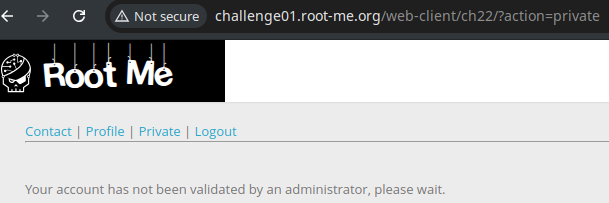
\includegraphics[scale=0.7]{private_before.png}
        \caption{Compte non-validé}
    \end{minipage}
    \begin{minipage}{0.45\textwidth}
        \centering
        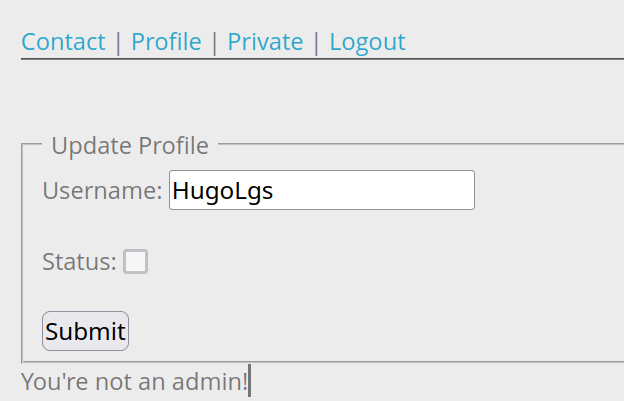
\includegraphics[scale=0.5]{not_admin.png}
        \caption{Nom d'utilisateur non-modifiable}
    \end{minipage}
    \caption{Premières constatations}
\end{figure}

Je me suis donc dit que je devais trouver un moyen de modifier ce formulaire pour "forcer" la validation de mon compte, où accéder à un rôle me permettant de le faire. J'ai d'abord testé depuis l'inspecteur pour voir ce que j'obtenais en modifiant le code du formulaire : 

\begin{figure}[!h]
	\centering
	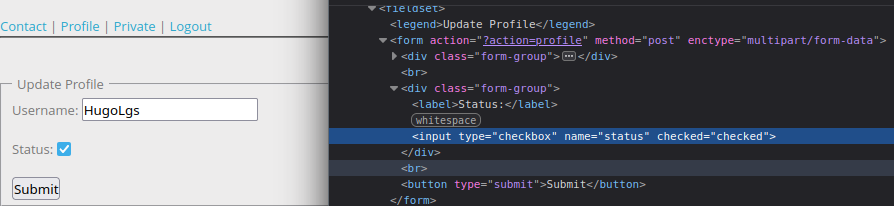
\includegraphics[scale=.5]{code_a_injecter.png}
	\caption{Code test}
\end{figure}

On peut voir qu'avec le \texttt{checked="checked"}, je pouvais modifier le formulaire pour m'approcher de ce que je souhaitais. 


Après quelques recherches sur le forum, j'ai compris qu'il était possible de mofidier ce formulaire injectant un code modifié directement dans la page où se situe ce formulaire. Pour cela, j'ai utilisé le formulaire pour contacter un admin du site. Dans la partie du \texttt{textarea}, j'ai entré le code suivant : 



J'ai pris ce code depuis le code source de la page profil, et je modifie ensuite ce dernier grâce à une injection en entrant le code suivi dans le formulaire de contact

\begin{figure}[!h]
	\centering
	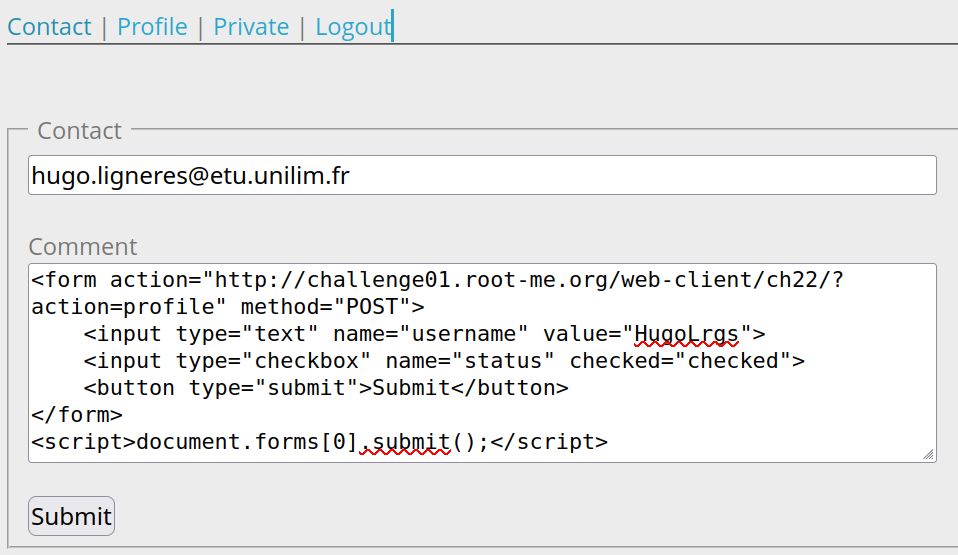
\includegraphics[scale=.45]{formulaire.png}
	\caption{Code à injecter}
\end{figure}
	
Dans les grandes lignes, ce code envoi une requête POST à l'url de la page pour modifier le nom d'utilisateur, en modifiant la checkbox avec \texttt{checked="checked"}. Ceci me permet de modifier le code source de la page ciblée, et d'y modifier le formulaire qui s'y trouve. \\

Une fois cette injection réalisée, la page "Private" a été modifiée, et le flag à entrer pour valider le challenge est affiché : 

\begin{figure}[!h]
	\centering
	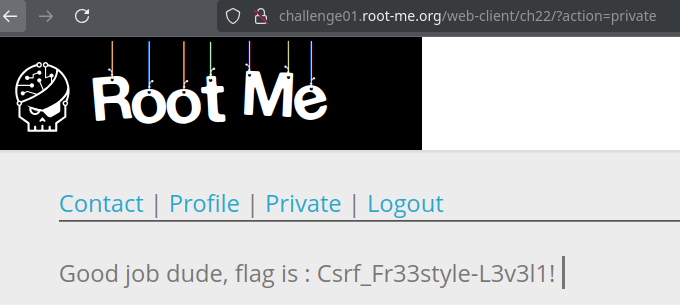
\includegraphics[scale=.45]{private_after.png}
	\caption{Flag affiché}
\end{figure}

Voici la preuve que le challenge a été validé : 

\begin{figure}[!h]
	\centering
	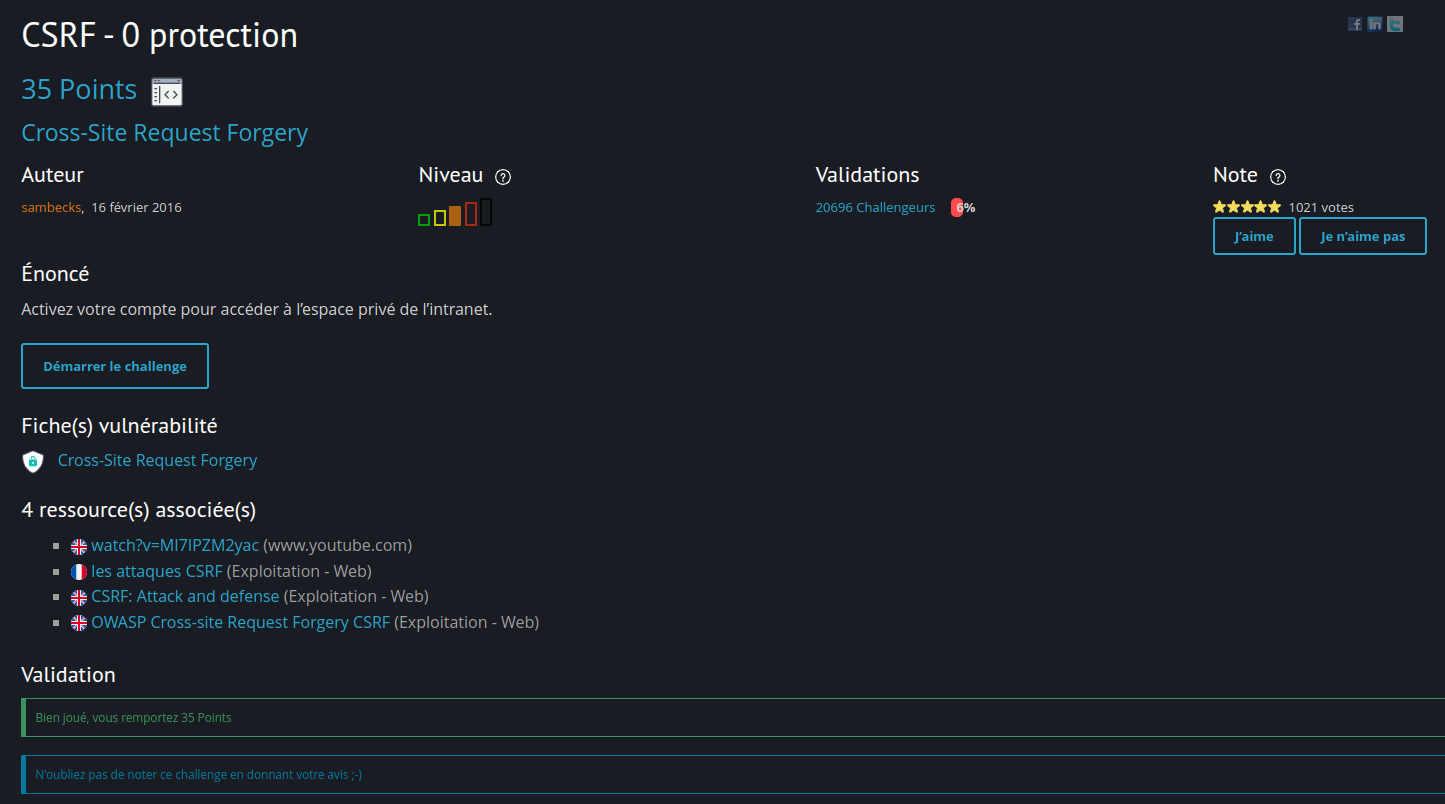
\includegraphics[scale=.45]{reussi_rootme.png}
	\caption{Challenge réussi}
\end{figure}

\newpage
	
	\subsection{CSRF - contournement de jeton}

\section{Partie 2 : XSS}

	\subsection{Challenge root-me}
	
	J'ai choisi de travailler sur le challenge \textbf{XSS DOM Based - Introduction}	
	
\begin{figure}[!h]
    \centering
    \begin{minipage}{0.45\textwidth}
        \centering
        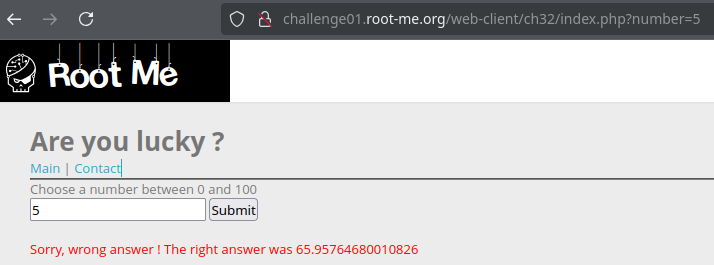
\includegraphics[scale=0.5]{xss_page_lucky_number.png}
        \caption{Page "Main"}
    \end{minipage}
    \begin{minipage}{0.45\textwidth}
        \centering
        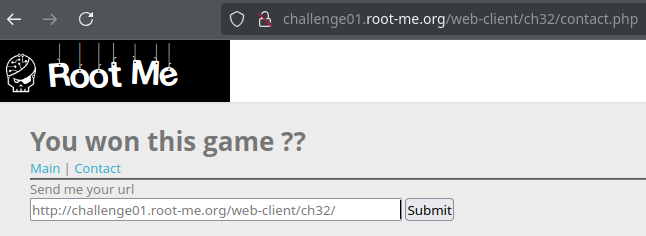
\includegraphics[scale=0.5]{xss_page_contact.png}
        \caption{Page "Contact"}
    \end{minipage}
    \caption{Les pages du challenge}
\end{figure}

(présenter ce que font les 2 pages)


J'ai dans un premier temps testé l'injection de code JavaScript très simple dans le formulaire du lucky number, car celui-ci n'imposait pas de format de données à entrer. Après différentes itérations tentées, j'ai obtenu ce code qui produisait l'effet attendu : un message d'alerte qui s'affichait quand on clique sur "Submit" : \texttt{test'; alert(1);//}

\begin{figure}[!h]
    \centering
    \begin{minipage}{0.45\textwidth}
        \centering
        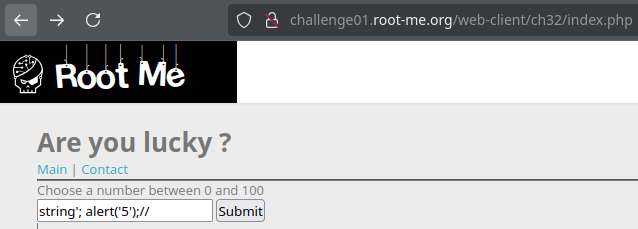
\includegraphics[scale=0.5]{xss_code_alert.png}
        \caption{Injection du code}
    \end{minipage}
    \begin{minipage}{0.45\textwidth}
        \centering
        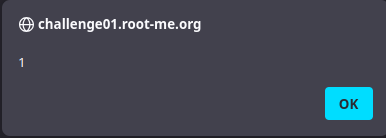
\includegraphics[scale=0.5]{alert.png}
        \caption{Résultat}
    \end{minipage}
    \caption{Premier test}
\end{figure}

Maintenant que

Ensuite, webhook 
	\subsection{Les recommandations ANSSI contre les vulnerabilités XSS}
	
	\textit{Expliquez les recommandations ANSSI contre les vulnerabilités XSS.}
	
	Encoder les données entrées, surtout celles entrées du côté client/navigateur d'une application
	Utiliser textContent ou l'API DOM pour manipuler le DOM, plutôt que des méthodes JavasCript qui injectent du code HTML, comme innerHTML par exemple. 
	
	
	
	Les pages HTML ne doivent pas contenir de code CSS ou JavaScript 
	
	

\end{document}
